\section{Results}

\subsection{Exploratory Data Analysis}

\begin{figure}[!htbp]
    \centering
    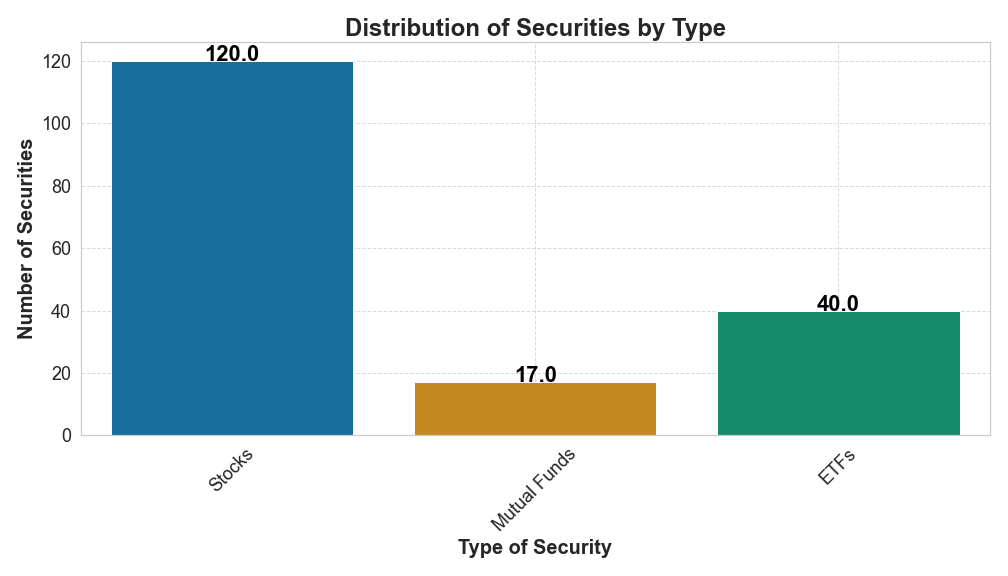
\includegraphics[width=0.7\textwidth]{../Figures/histogram_security_count.png}
    \caption{Distribution of Securities by Type}
    \label{fig:distribution_of_securities}
    \subcaption{This figure illustrates the distribution of different types of securities within the dataset. It shows that stocks make up the majority with 120 securities, followed by ETFs with 40, and mutual funds with 17.}
\end{figure}
\FloatBarrier

\begin{figure}[!htbp]
    \centering
    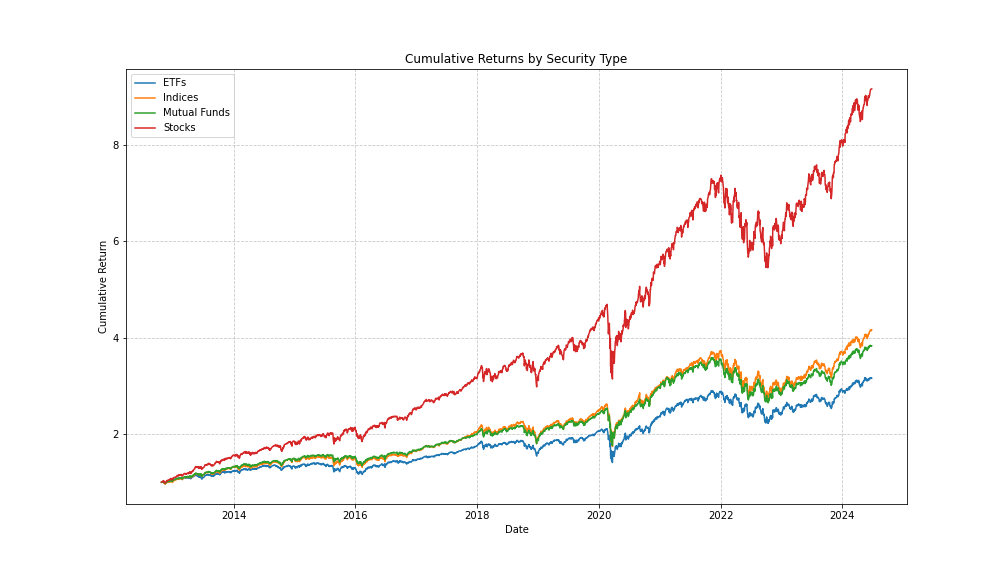
\includegraphics[width=0.7\textwidth]{../Figures/cumulative_returns_by_type.png}
    \caption{Cumulative Returns Over Time by Security Type}
    \label{fig:cumulative_returns_by_type}
    \subcaption{Stocks exhibit the highest cumulative return over time, indicating a higher potential for long-term growth compared to ETFs and mutual funds. ETFs and mutual funds also show consistent returns, highlighting their role in diversified investment strategies.}
\end{figure}
\FloatBarrier

\subsection{Assets by Composite Score}

\begin{figure}[!htbp]
    \centering
    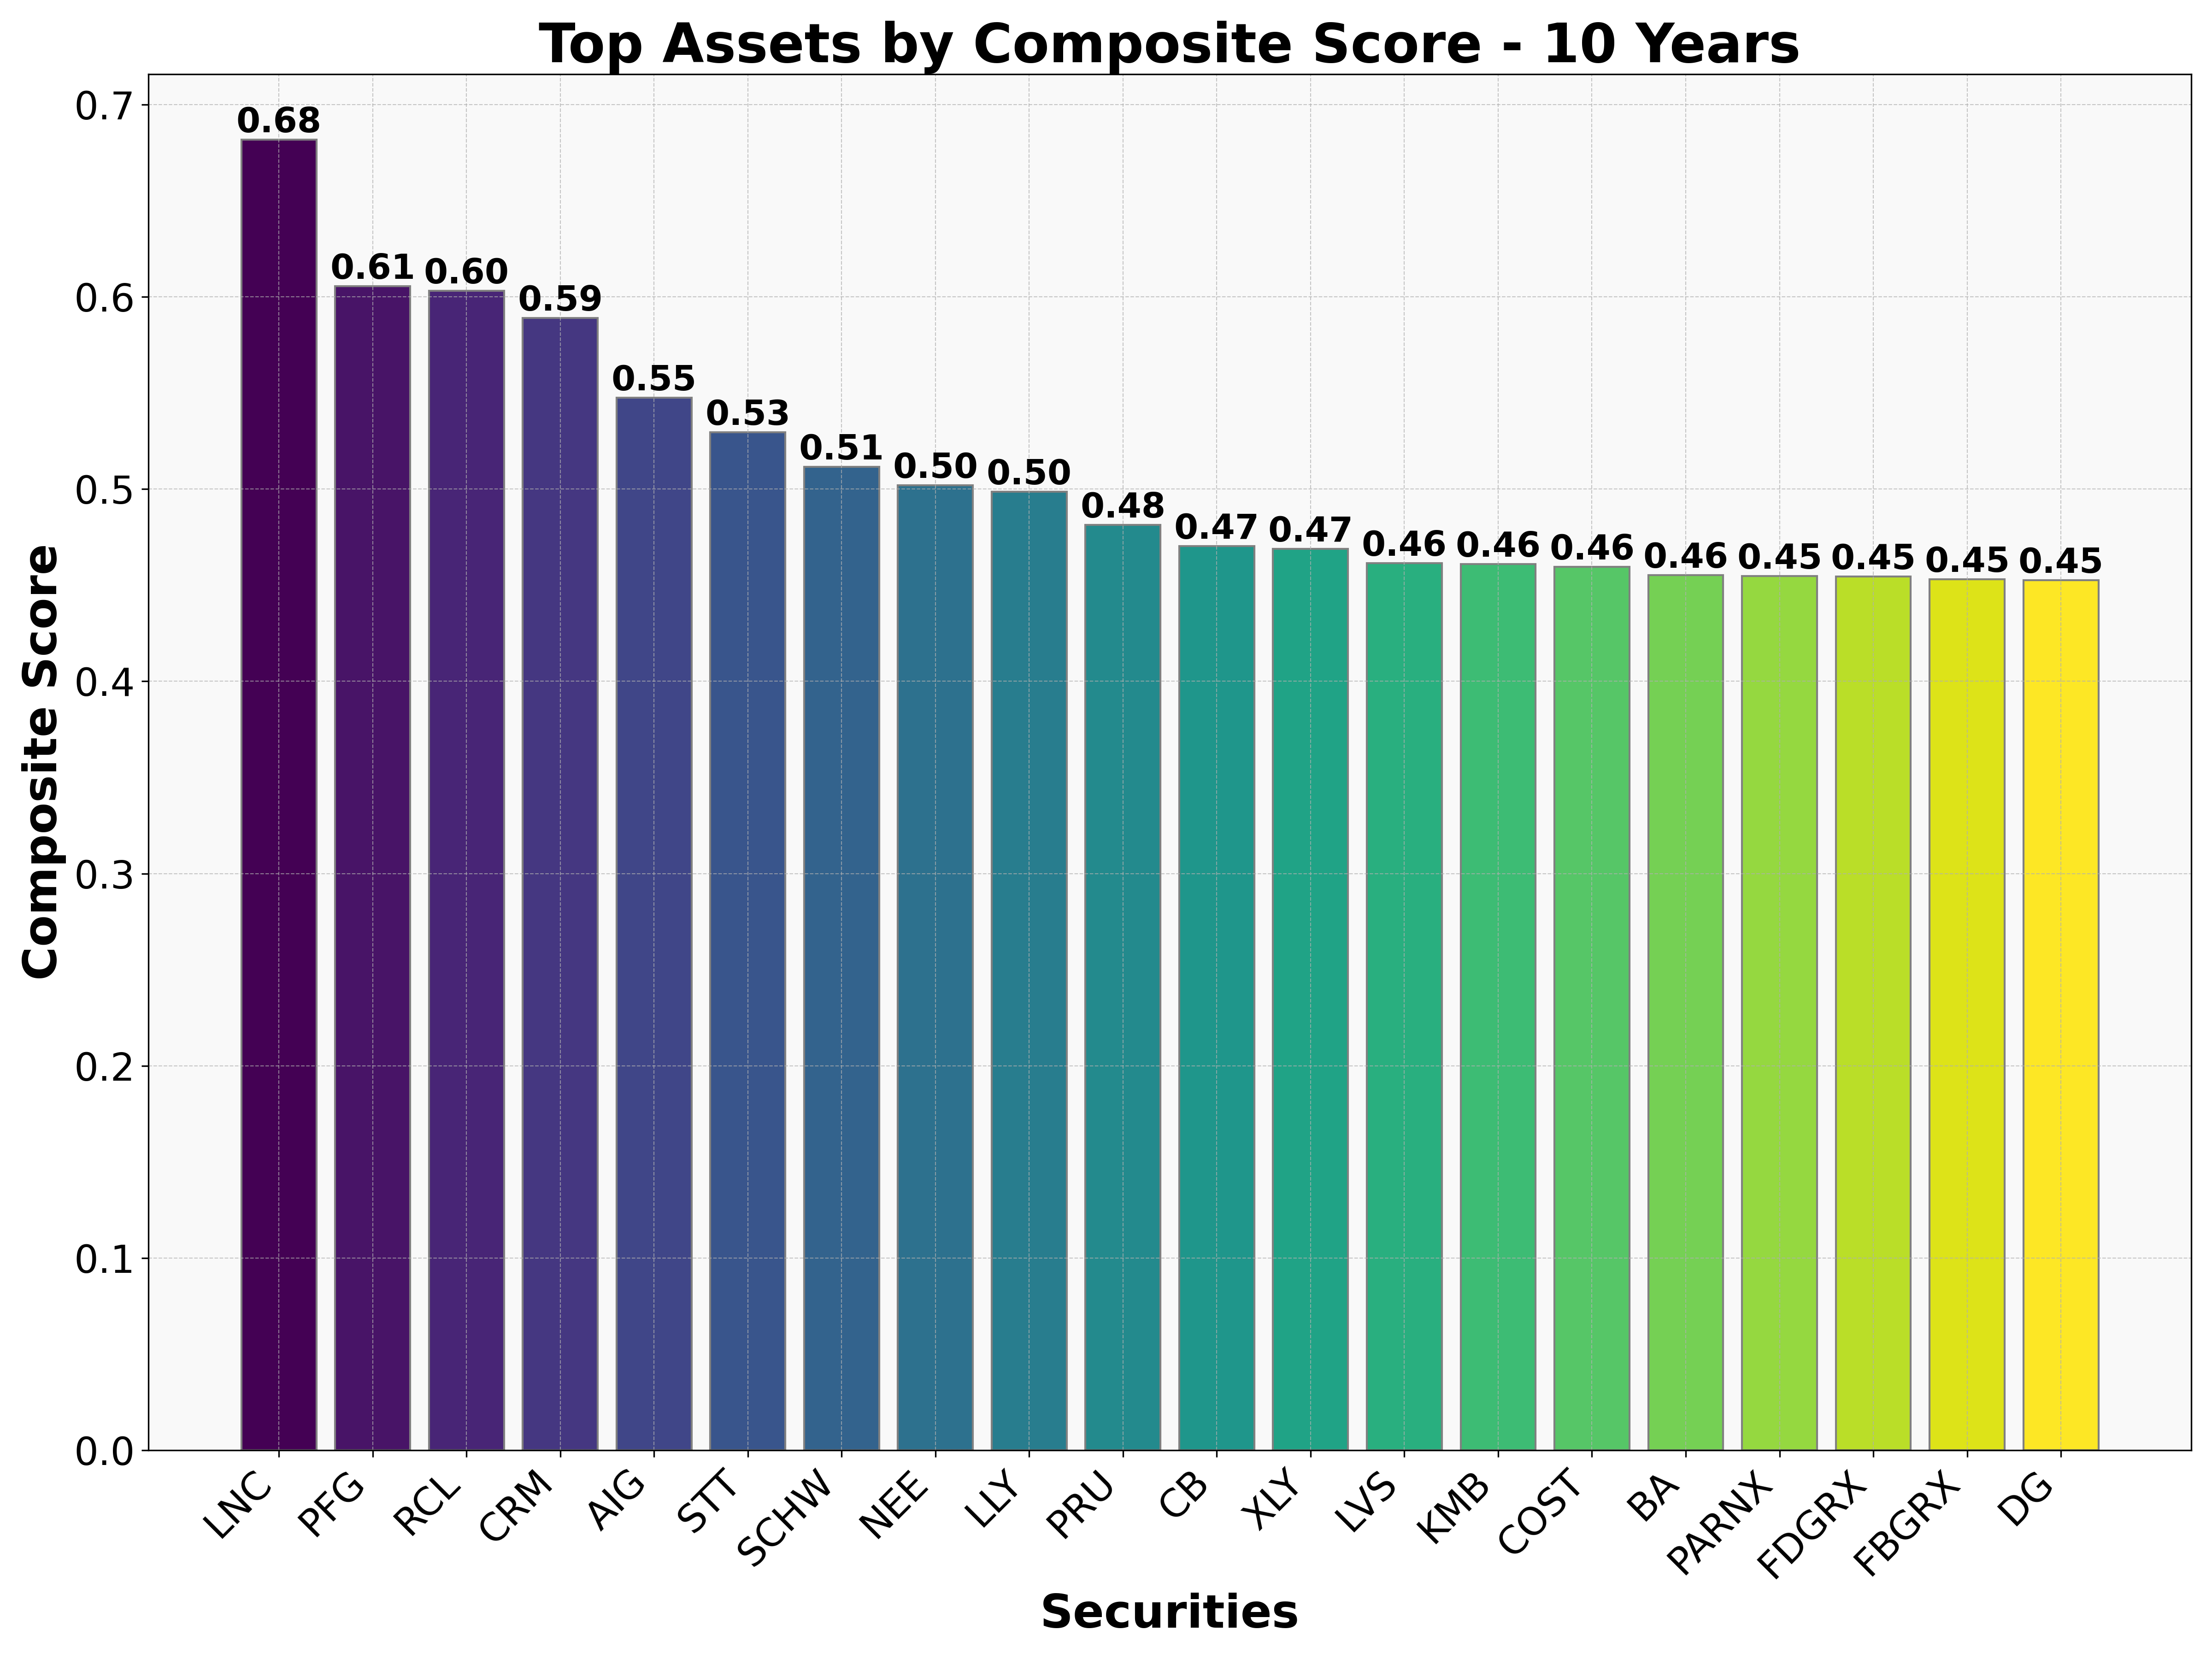
\includegraphics[width=0.7\textwidth]{../Figures/top_assets_composite_score_10_years.png}
    \caption{Top Assets by Composite Score (10 Years)}
    \label{fig:top_assets_10y}
    \subcaption{LNC, PFG, and RCL lead the rankings for the 10-year horizon, demonstrating their strong and consistent performance over a decade.}
\end{figure}
\FloatBarrier

\begin{figure}[!htbp]
    \centering
    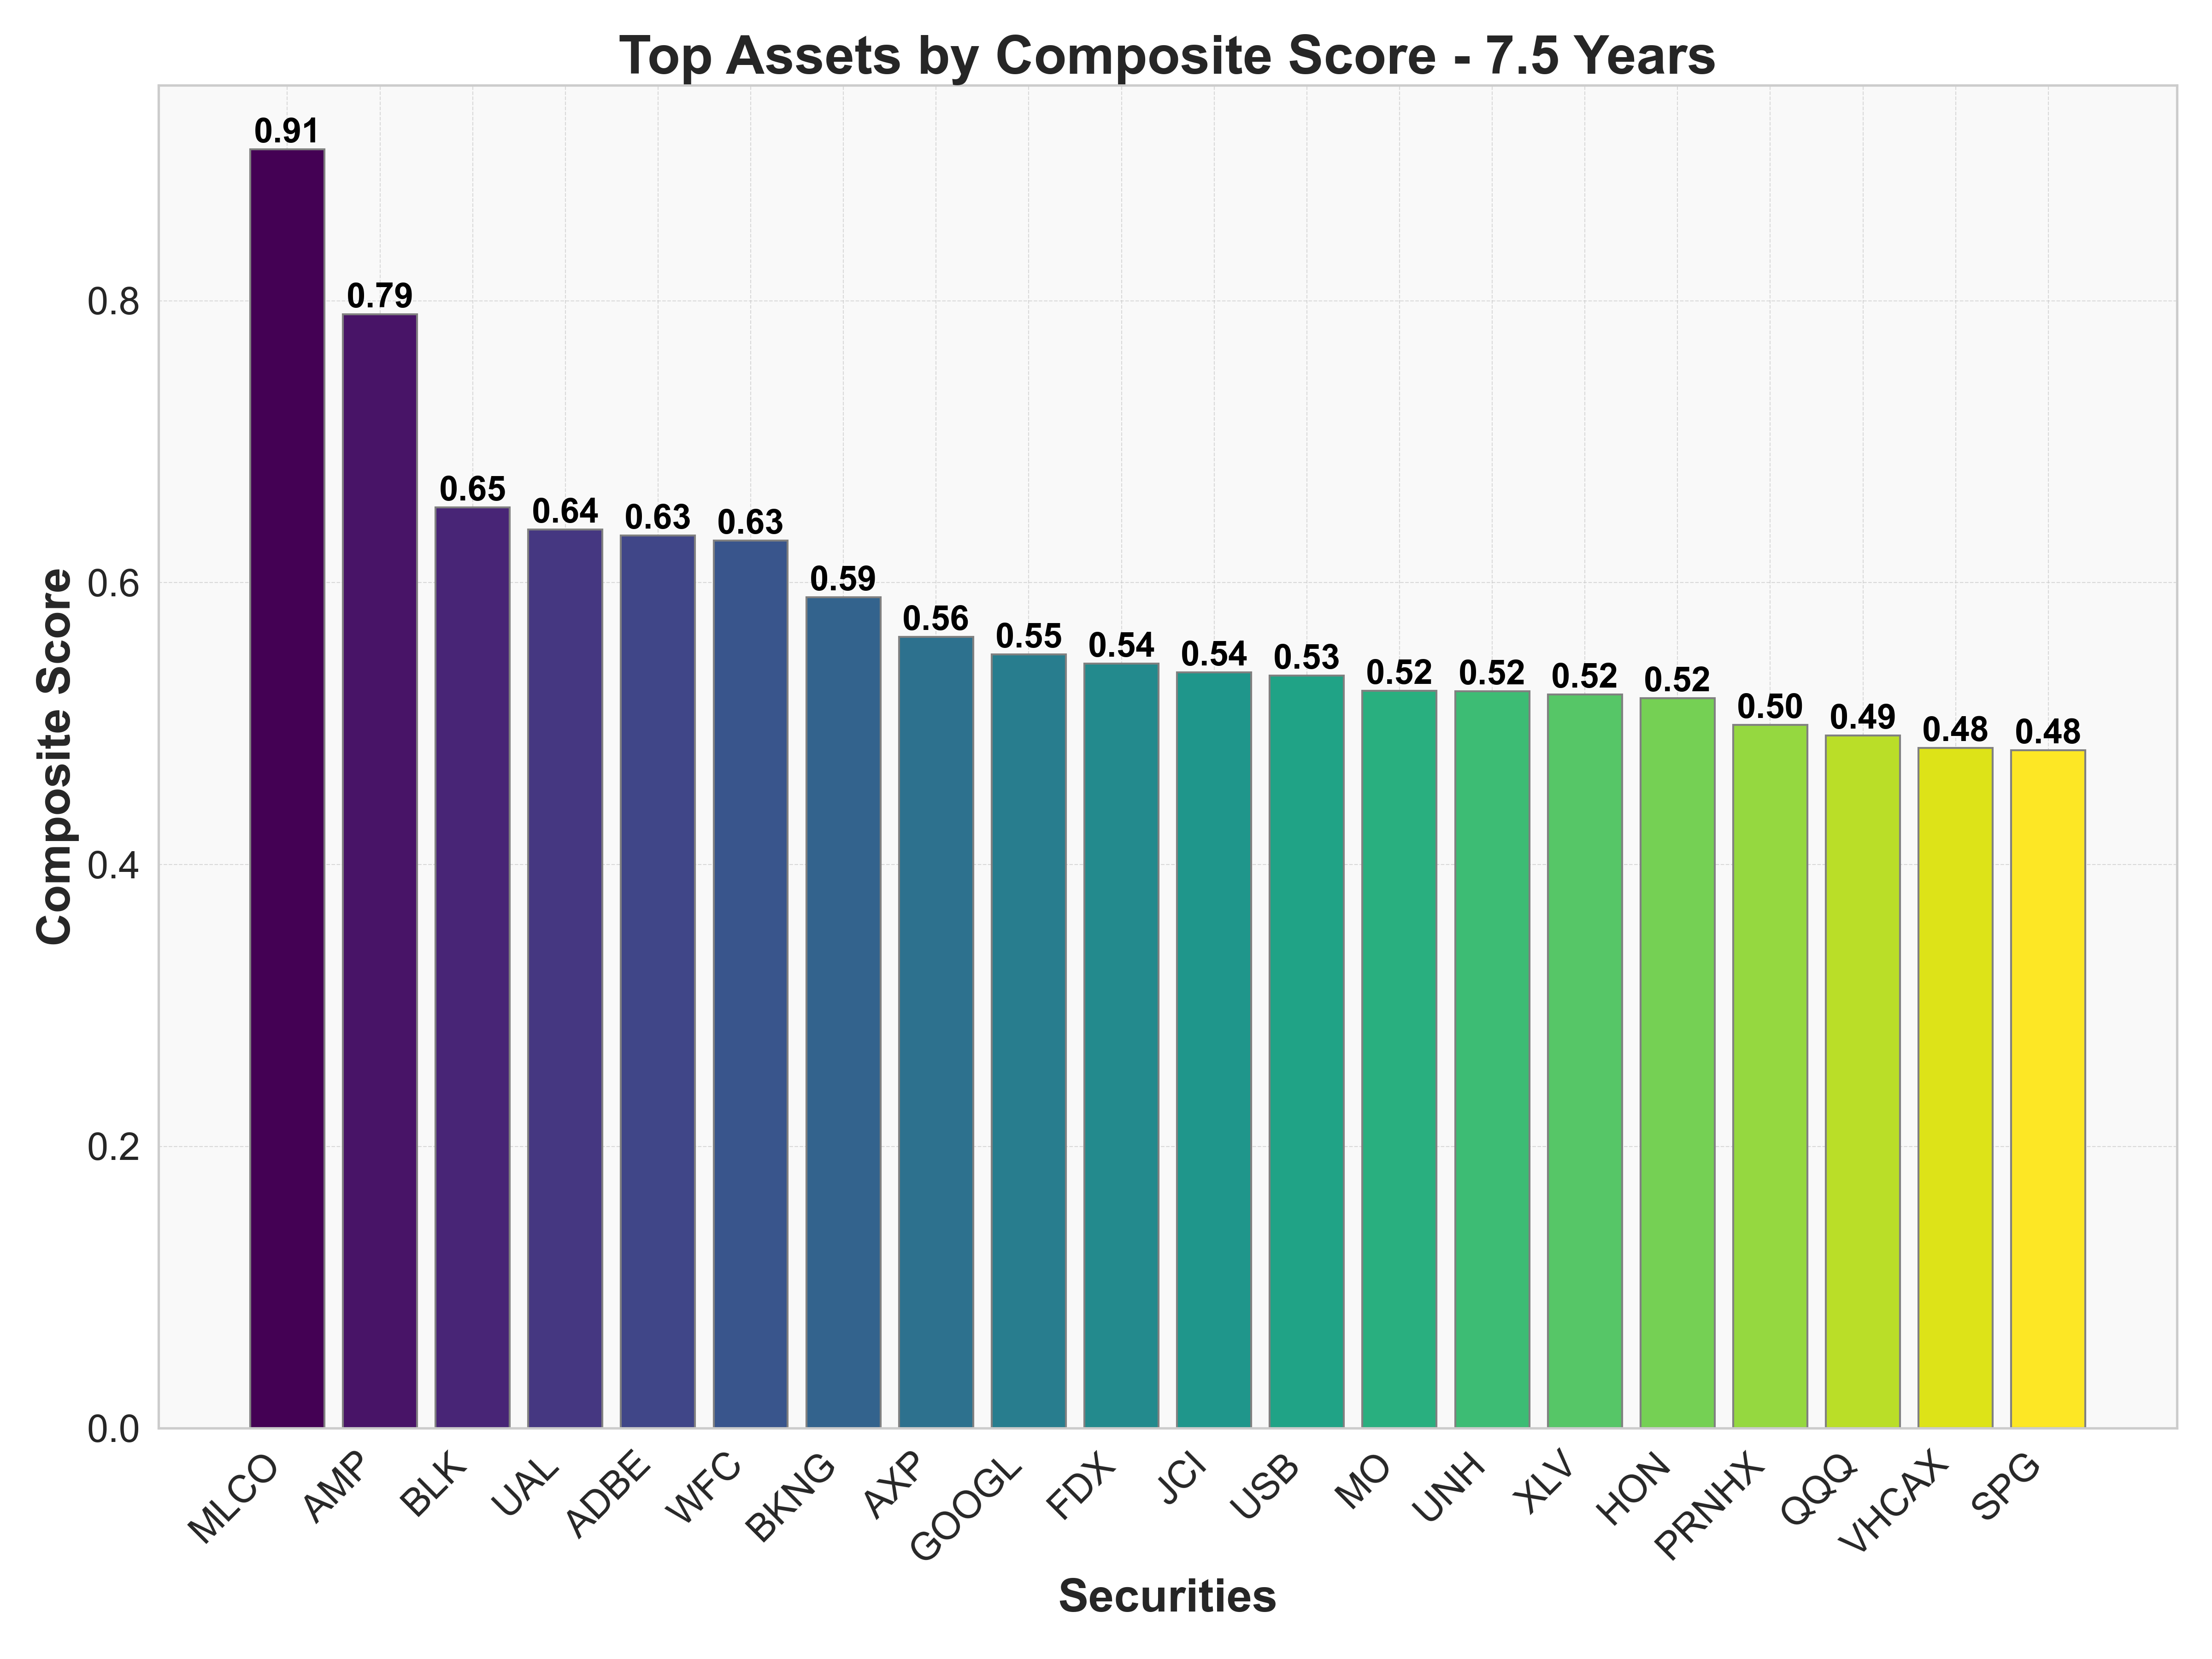
\includegraphics[width=0.7\textwidth]{../Figures/top_assets_composite_score_7_5_years.png}
    \caption{Top Assets by Composite Score (7.5 Years)}
    \label{fig:top_assets_7_5y}
    \subcaption{Over a 7.5-year horizon, MLCO, AMP, and BLK emerge as top assets, showcasing robust performance and highlighting their resilience in the market.}
\end{figure}
\FloatBarrier

\begin{figure}[!htbp]
    \centering
    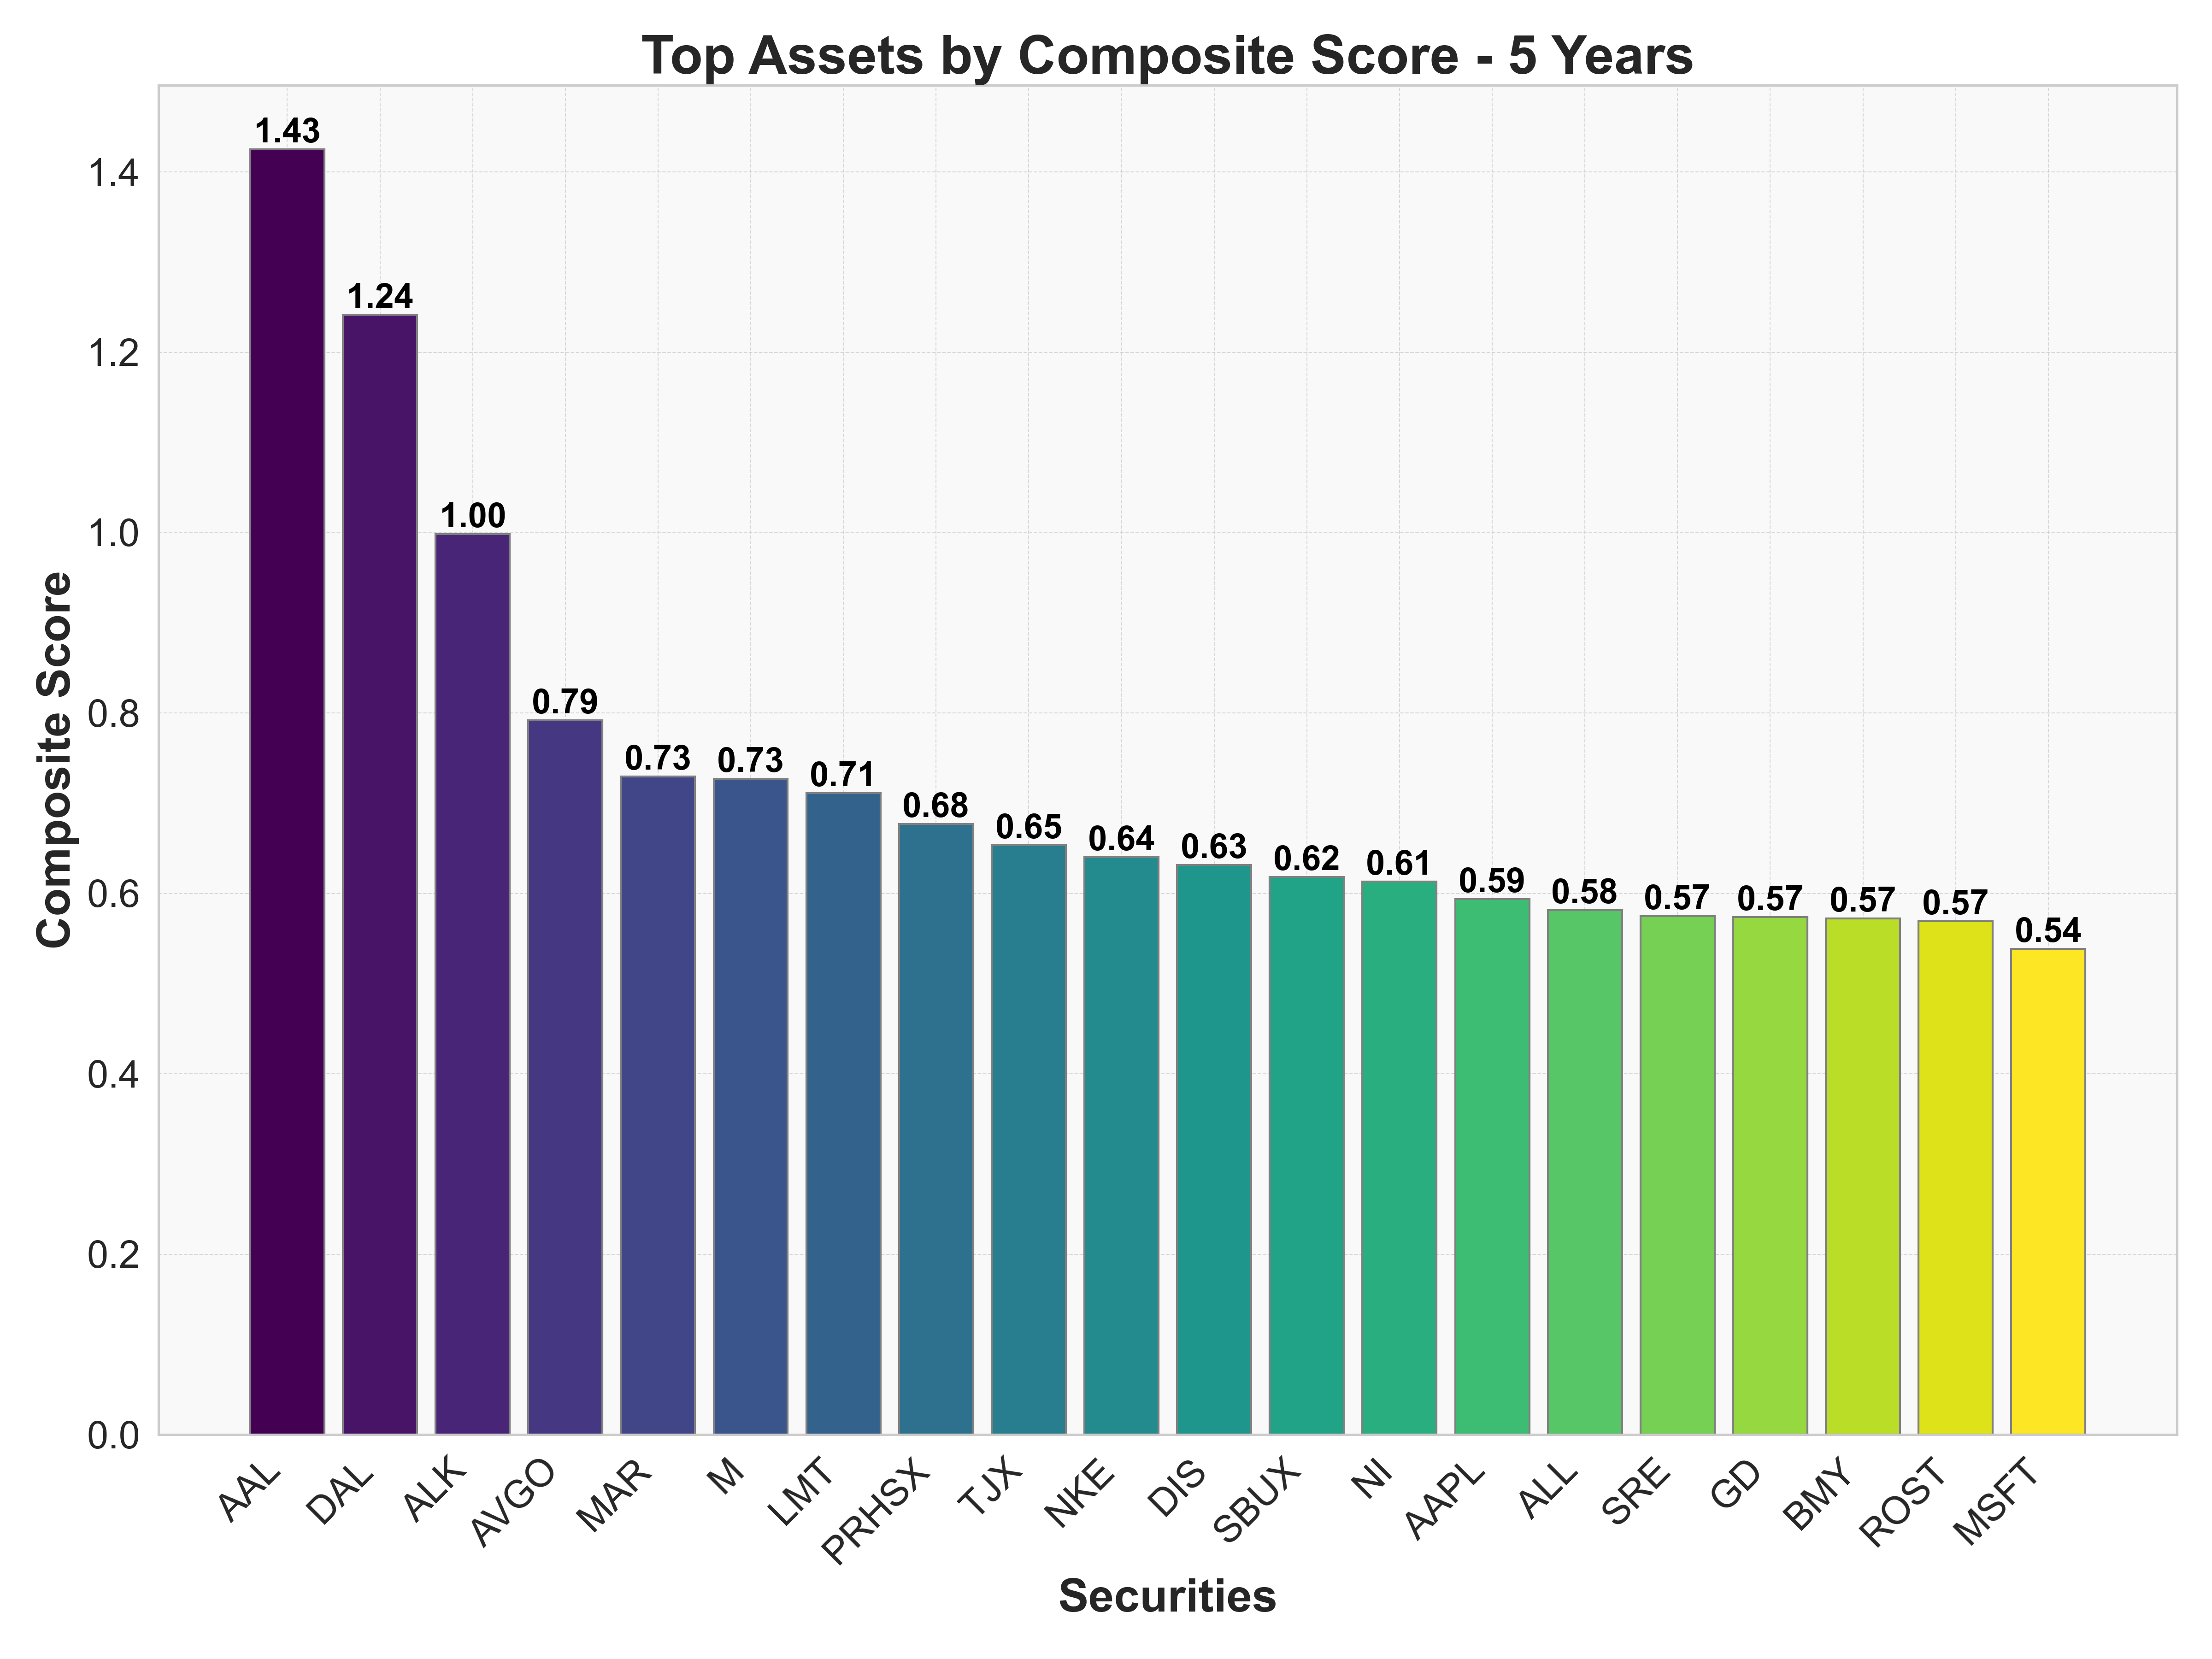
\includegraphics[width=0.7\textwidth]{../Figures/top_assets_composite_score_5_years.png}
    \caption{Top Assets by Composite Score (5 Years)}
    \label{fig:top_assets_5y}
    \subcaption{The top-performing assets over a 5-year horizon, ranked by composite score, include AAL, DAL, and ALK, reflecting a strong performance in the airline industry during this period.}
\end{figure}
\FloatBarrier

\subsection{Optimal Portfolios with Weights}

\begin{figure}[!htbp]
    \centering
    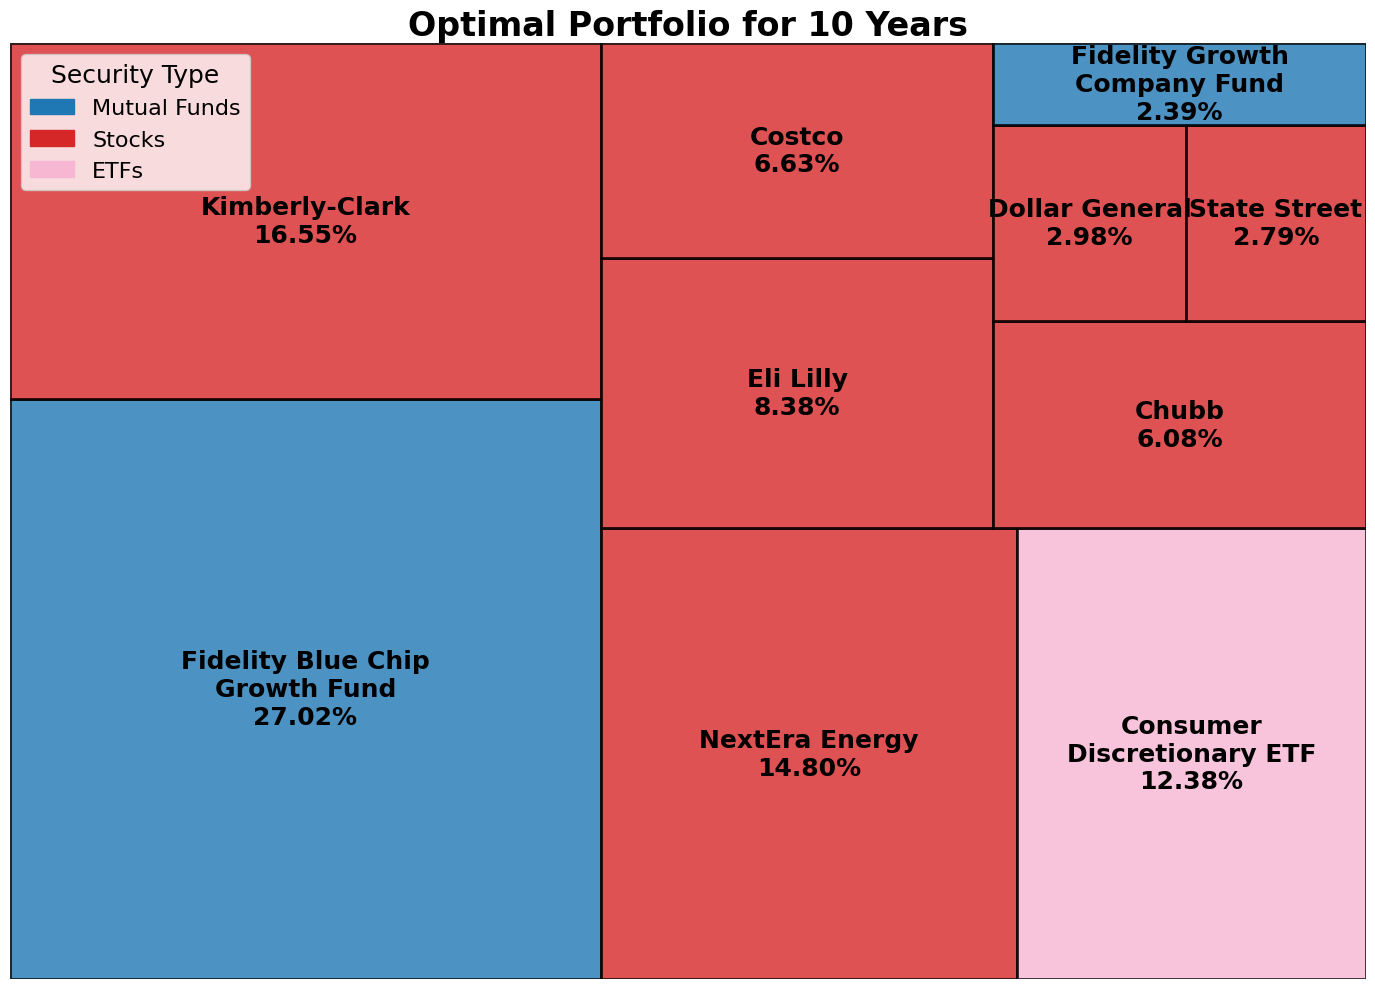
\includegraphics[width=0.7\textwidth]{../Figures/optimal_portfolio_10_years.png}
    \caption{Optimal Portfolio for 10 Years}
    \label{fig:optimal_portfolio_10y}
    \subcaption{This figure illustrates the optimal portfolio allocation for a 10-year investment horizon, showing the proportion of stocks, mutual funds, and ETFs. The portfolio is designed to maximize returns while managing risk over the long term.}
\end{figure}
\FloatBarrier

\begin{figure}[!htbp]
    \centering
    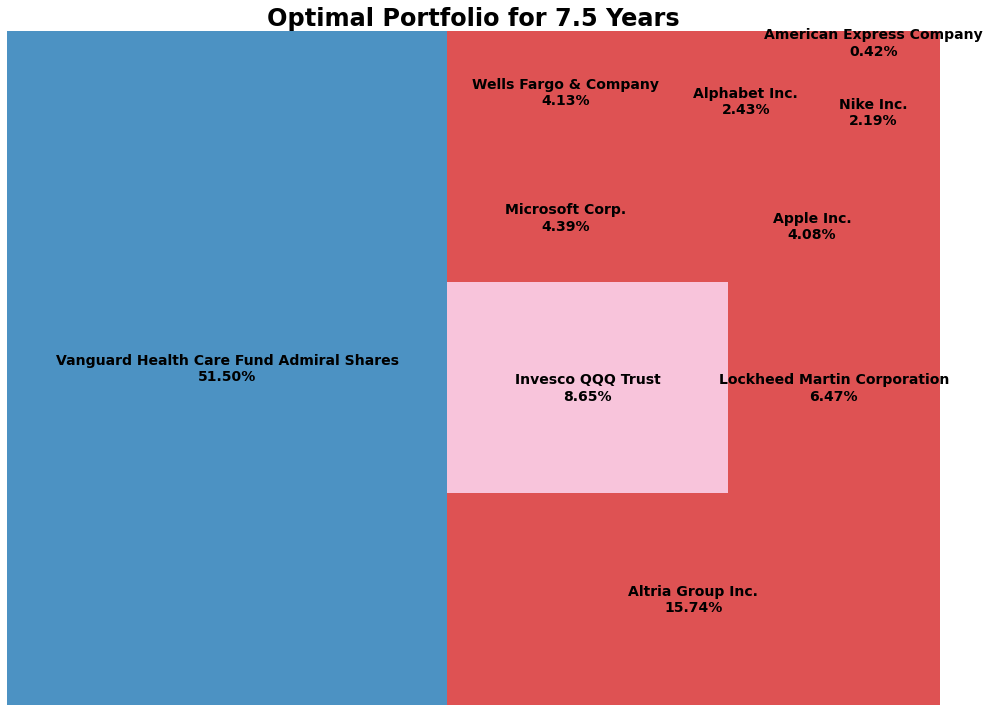
\includegraphics[width=0.7\textwidth]{../Figures/optimal_portfolio_7_5_years.png}
    \caption{Optimal Portfolio for 7.5 Years}
    \label{fig:optimal_portfolio_7_5y}
\end{figure}
\FloatBarrier

\begin{figure}[!htbp]
    \centering
    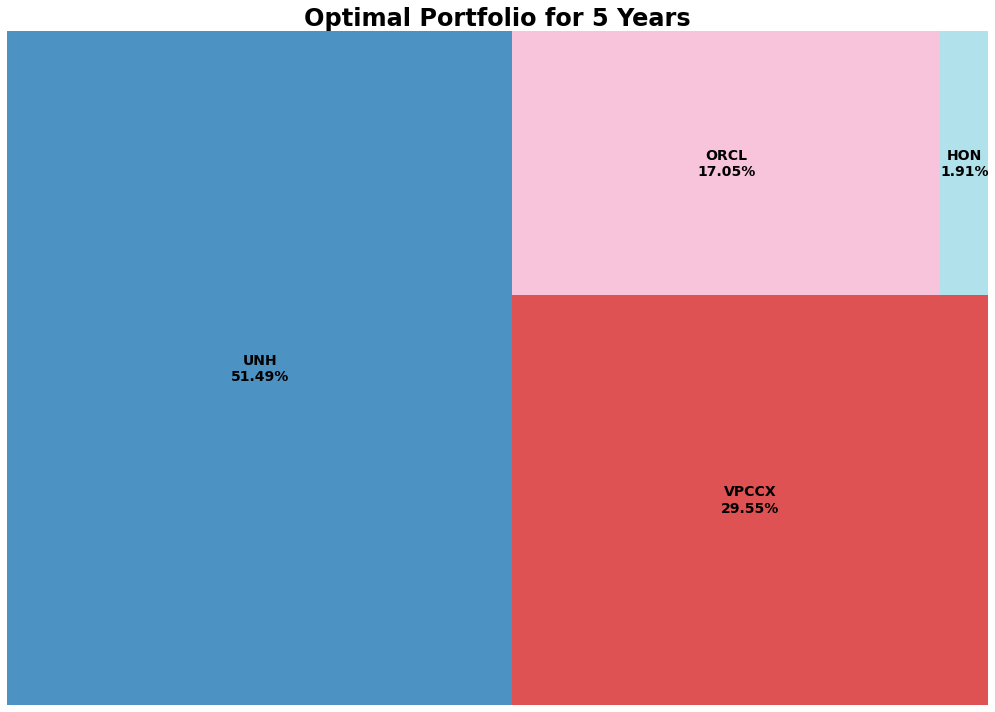
\includegraphics[width=0.7\textwidth]{../Figures/optimal_portfolio_5_years.png}
    \caption{Optimal Portfolio for 5 Years}
    \label{fig:optimal_portfolio_5y}
\end{figure}
\FloatBarrier

\subsection{Comparison with Hindsight Data}

\begin{figure}[!htbp]
    \centering
    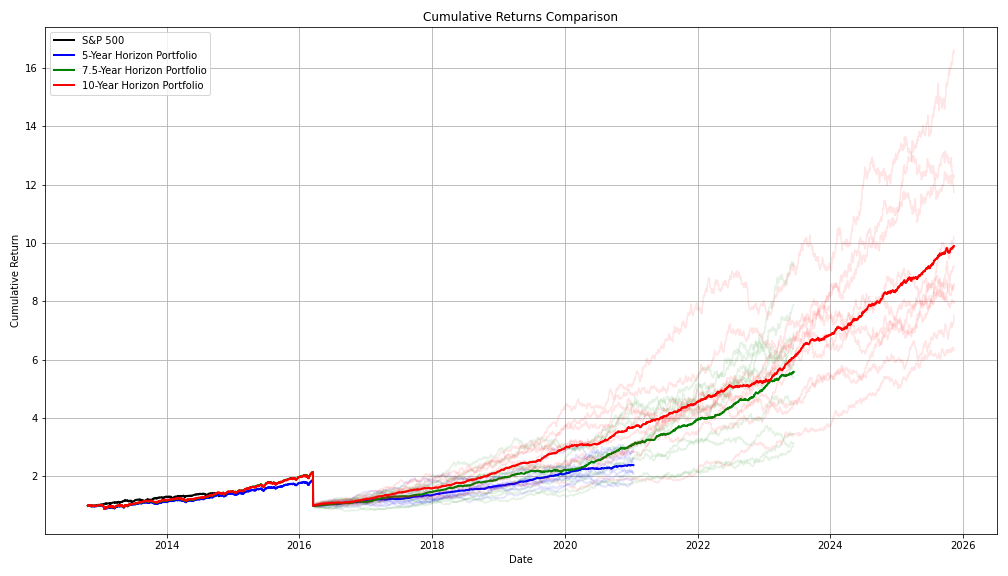
\includegraphics[width=0.7\textwidth]{../Figures/cumulative_returns_comparison.png}
    \caption{Cumulative Returns Comparison of Actual Portfolios vs. S\&P 500}
    \label{fig:cumulative_returns_comparison}
    \subcaption{This figure compares the cumulative returns of actual portfolios with the S\&P 500 benchmark. The results show that the actual portfolios for 5, 7.5, and 10-year horizons consistently outperform the S\&P 500, highlighting the effectiveness of the optimization strategy.}
\end{figure}
\FloatBarrier

\begin{figure}[!htbp]
    \centering
    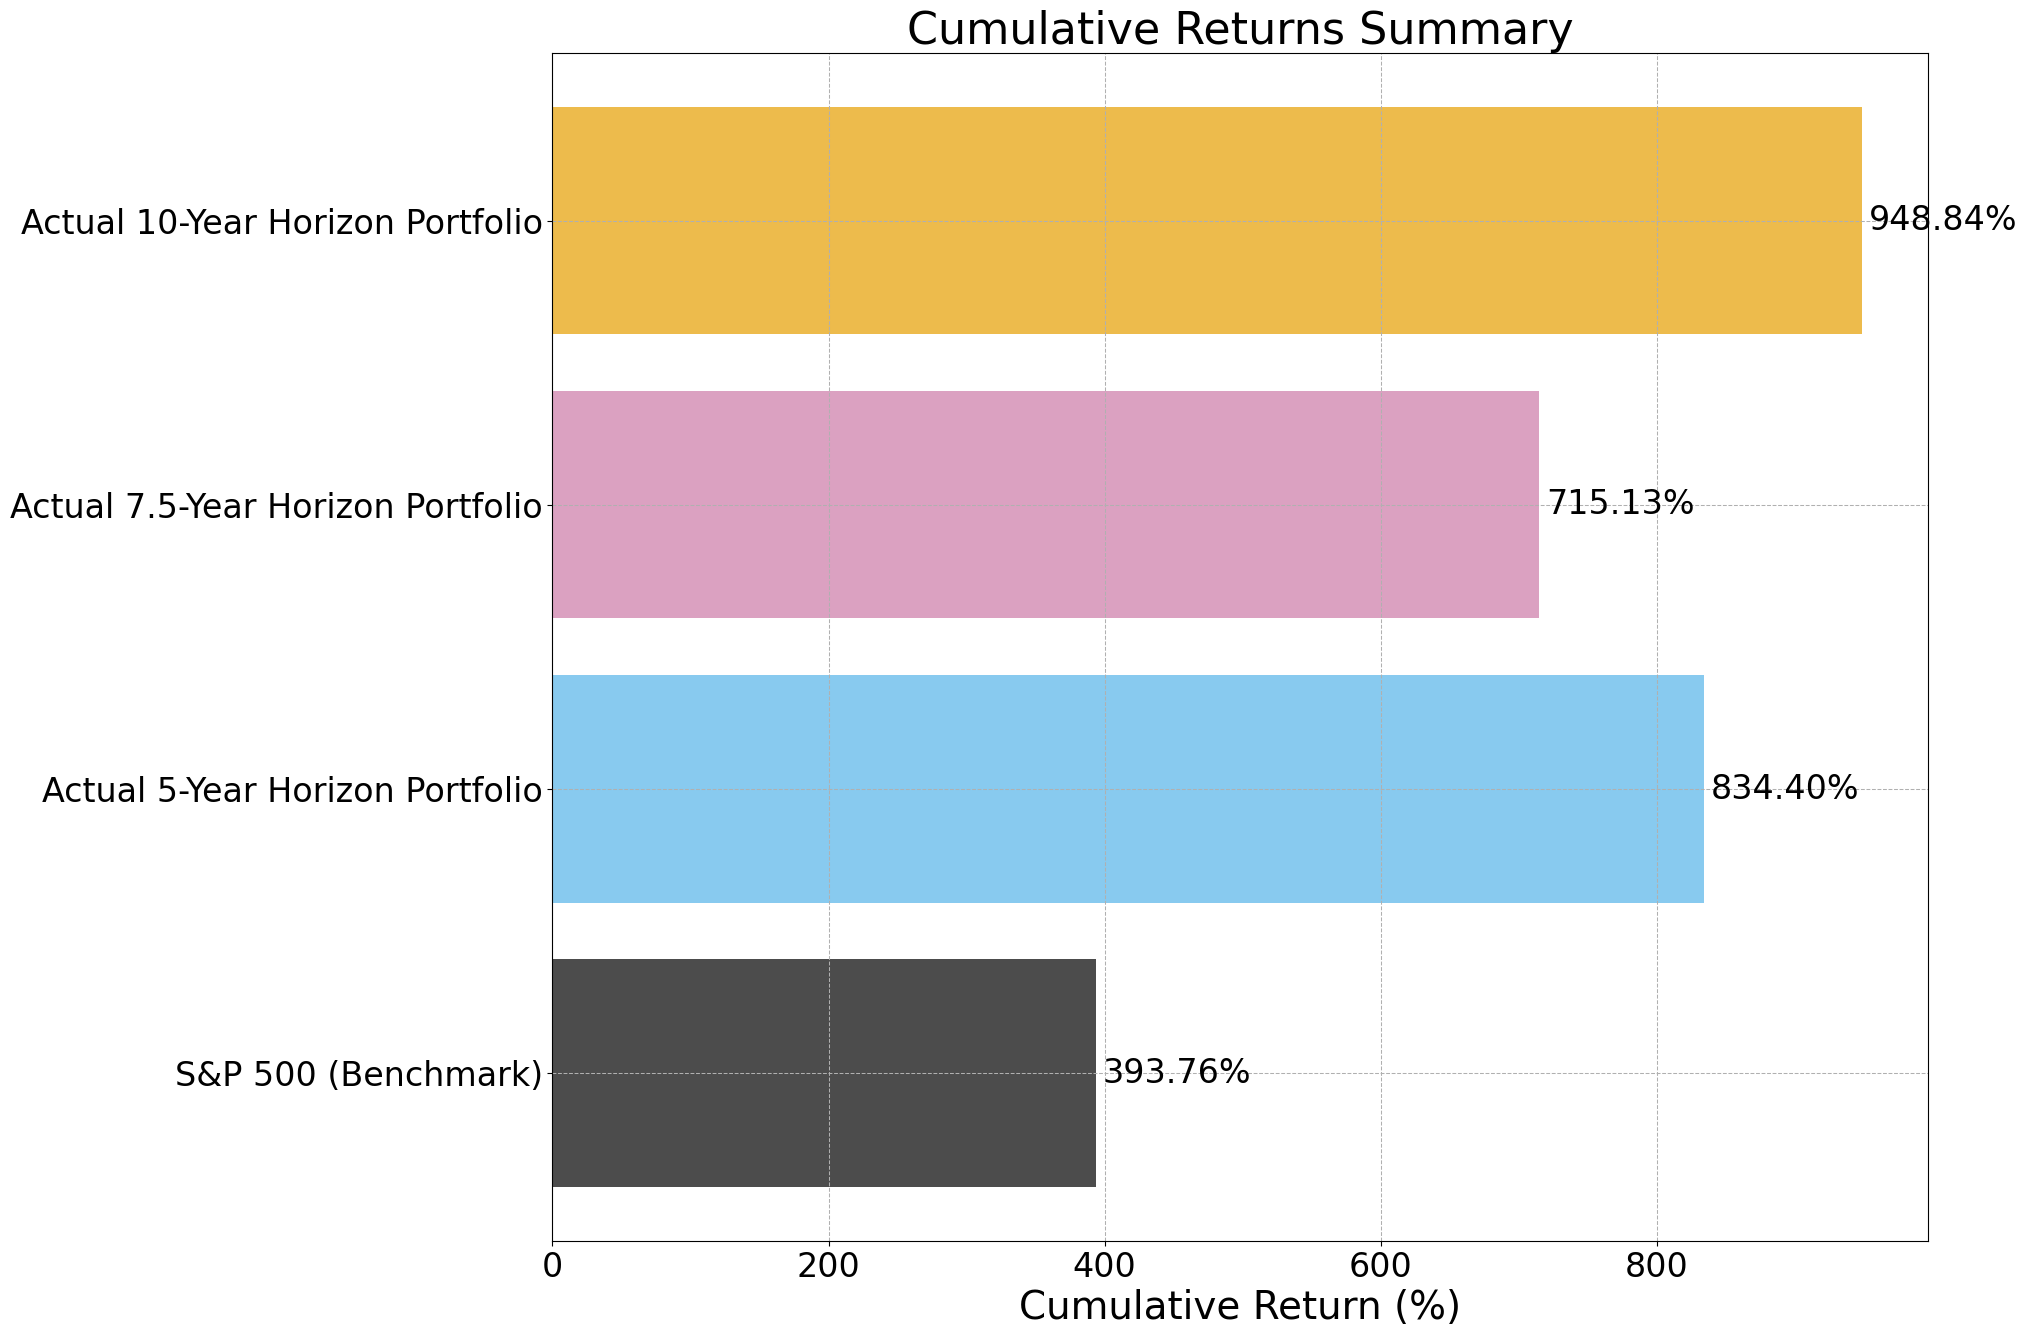
\includegraphics[width=0.7\textwidth]{../Figures/cumulative_returns_summary.png}
    \caption{Cumulative Returns Summary}
    \label{fig:cumulative_returns_summary}
    \subcaption{This summary illustrates the cumulative returns for the 5, 7.5, and 10-year horizon portfolios compared to the S\&P 500 benchmark.}
\end{figure}
\FloatBarrier

\subsection{Forecasting Results Using Monte Carlo}

\begin{figure}[!htbp]
    \centering
    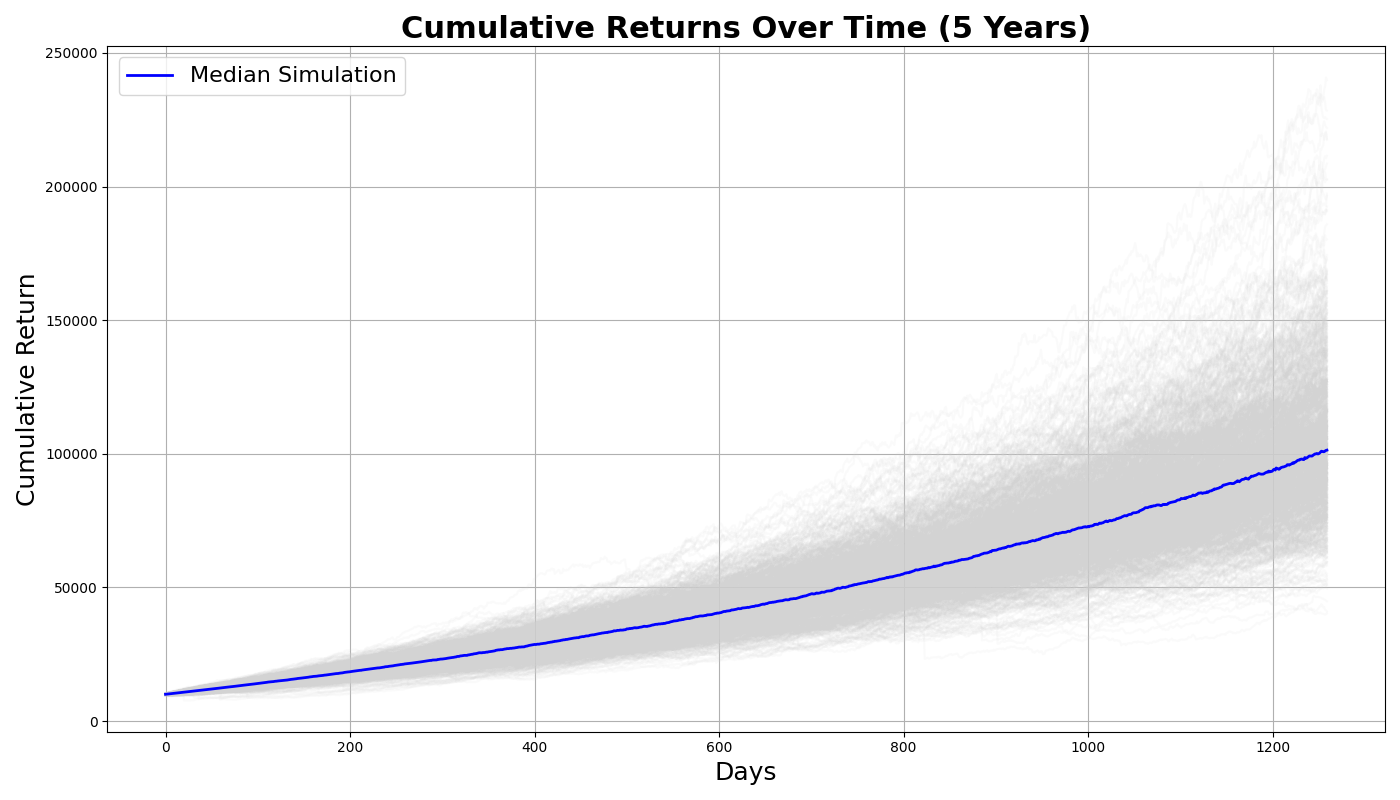
\includegraphics[width=0.8\textwidth]{../Figures/cumulative_returns_over_time_5_years.png}
    \caption{Cumulative Returns Over Time (5 Years)}
    \label{fig:cumulative_returns_5y}
    \subcaption{This figure shows the cumulative returns over a 5-year period. The blue line represents the median simulation of portfolio returns, with the gray lines indicating the range of possible outcomes from the Monte Carlo simulations.}
\end{figure}
\FloatBarrier

\begin{figure}[!htbp]
    \centering
    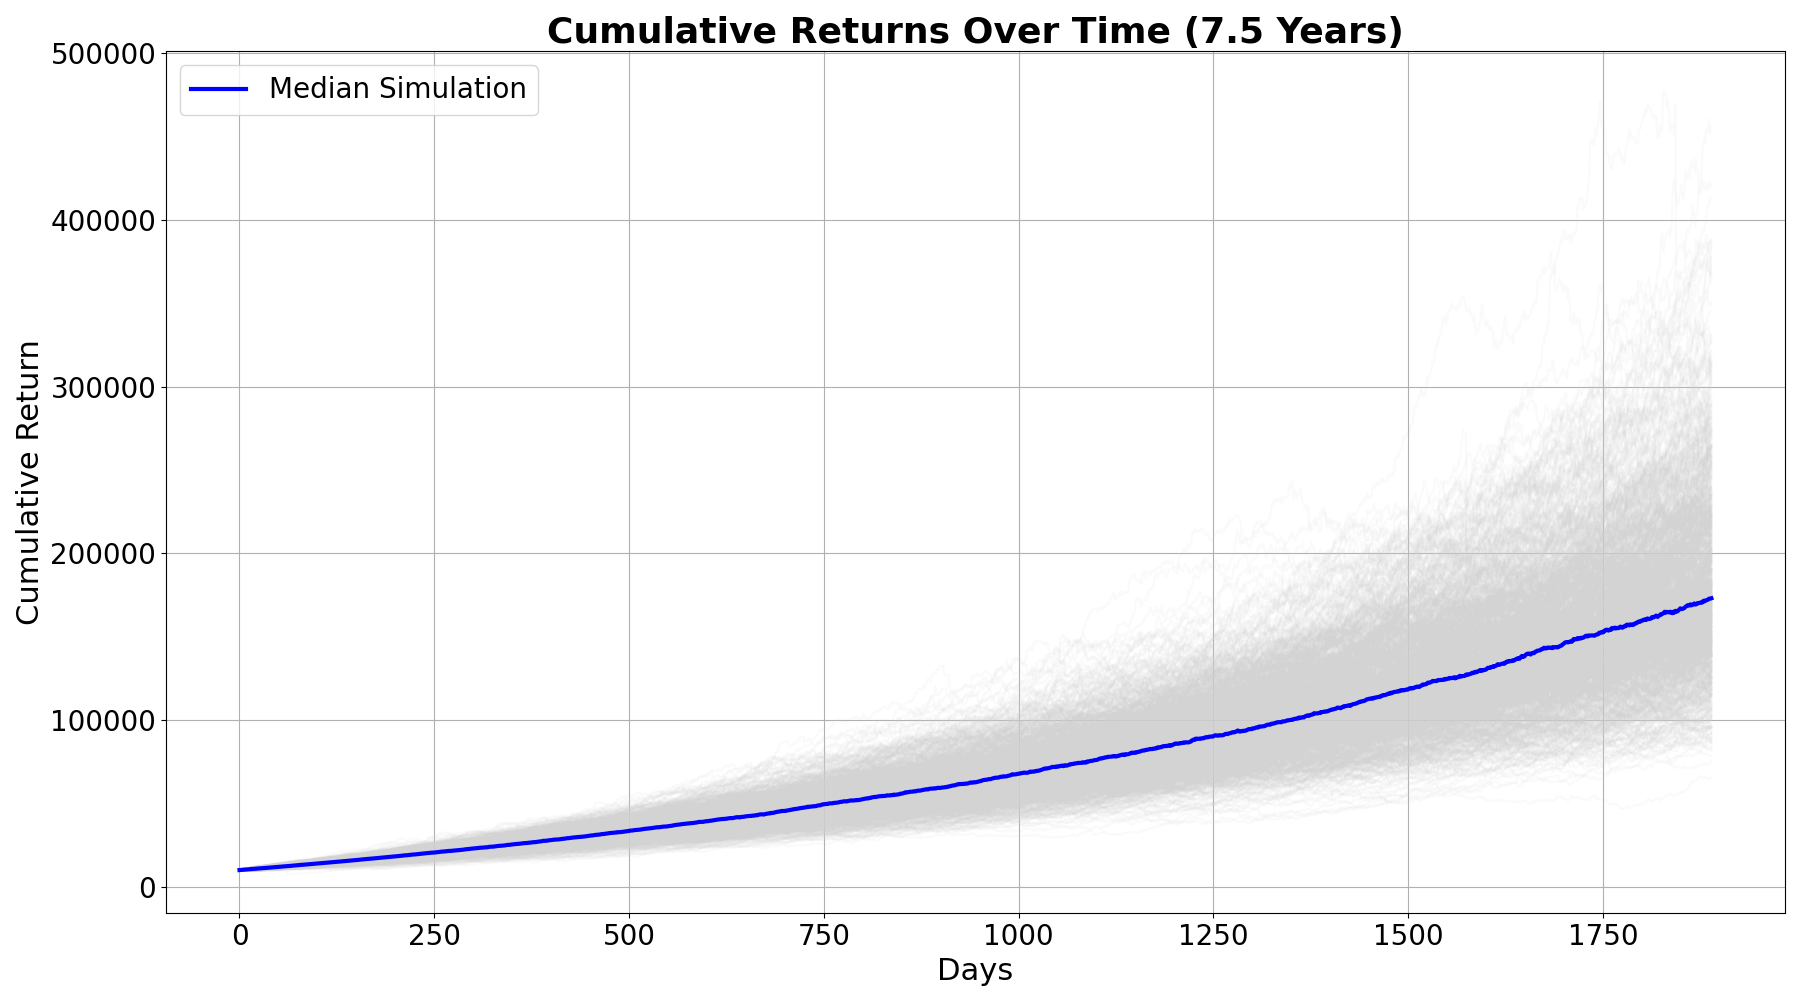
\includegraphics[width=0.8\textwidth]{../Figures/cumulative_returns_over_time_7_5_years.png}
    \caption{Cumulative Returns Over Time (7.5 Years)}
    \label{fig:cumulative_returns_7_5y}
\end{figure}
\FloatBarrier

\begin{figure}[!htbp]
    \centering
    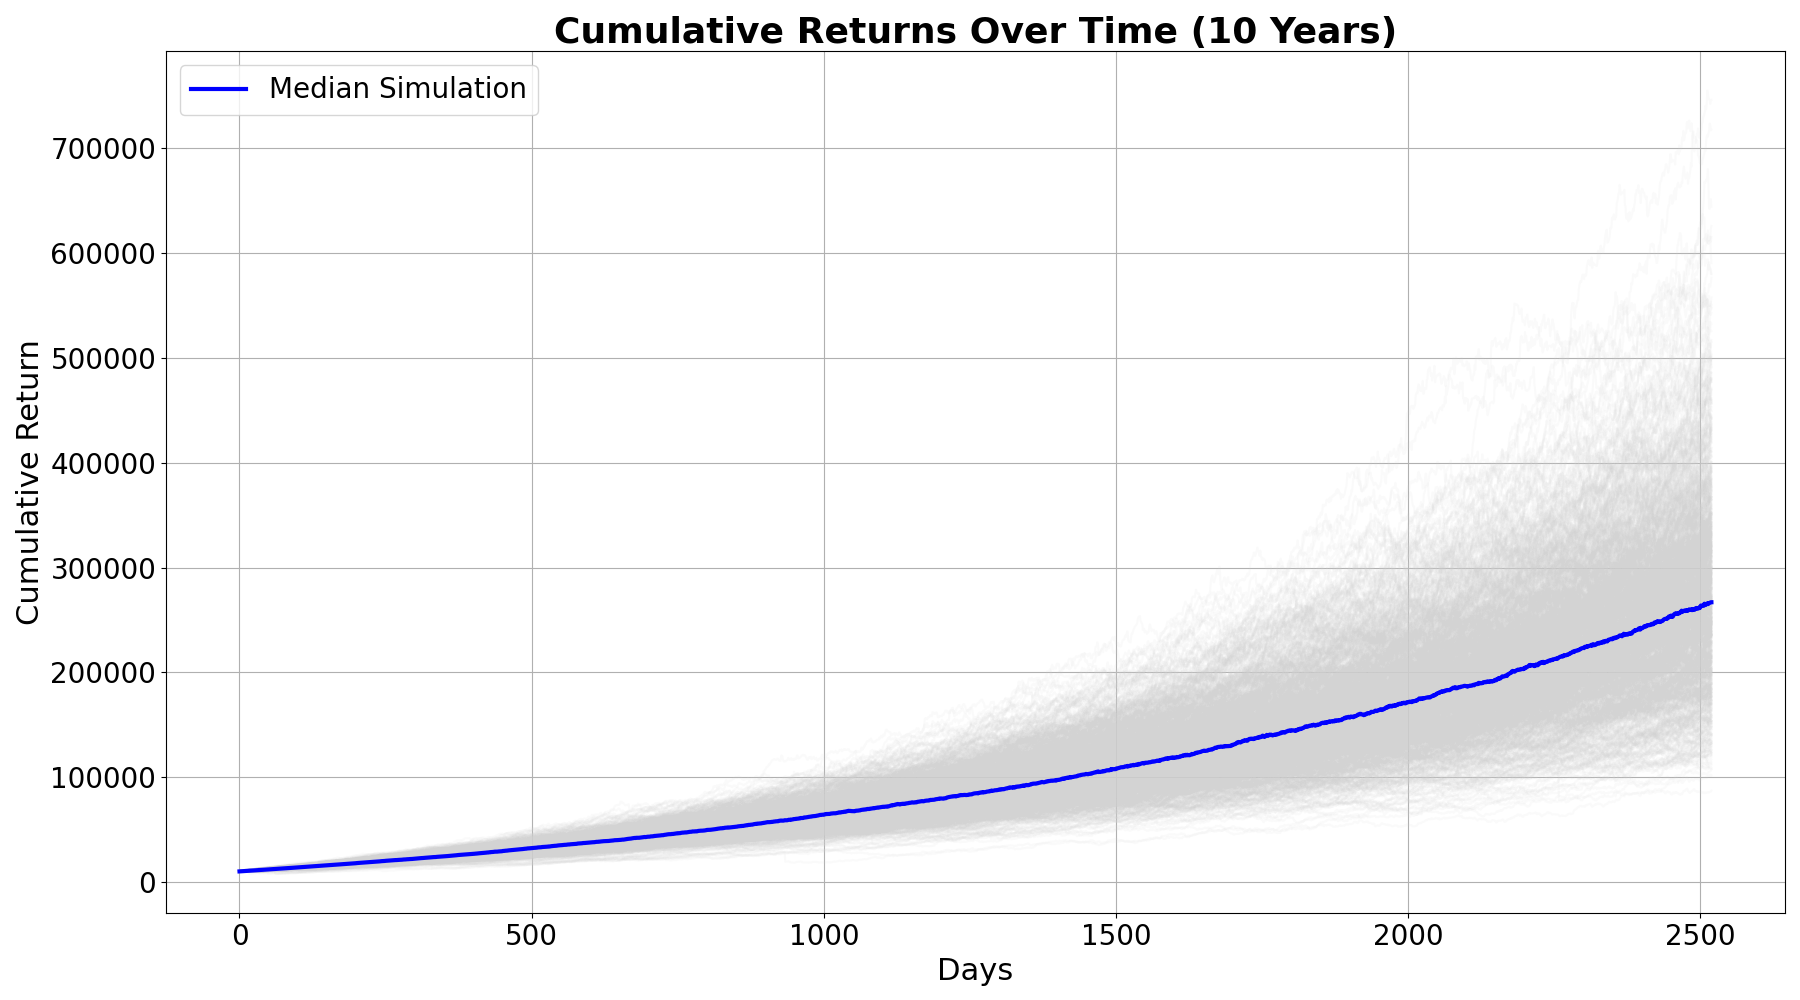
\includegraphics[width=0.8\textwidth]{../Figures/cumulative_returns_over_time_10_years.png}
    \caption{Cumulative Returns Over Time (10 Years)}
    \label{fig:cumulative_returns_10y}
\end{figure}
\FloatBarrier

\begin{figure}[!htbp]
    \centering
    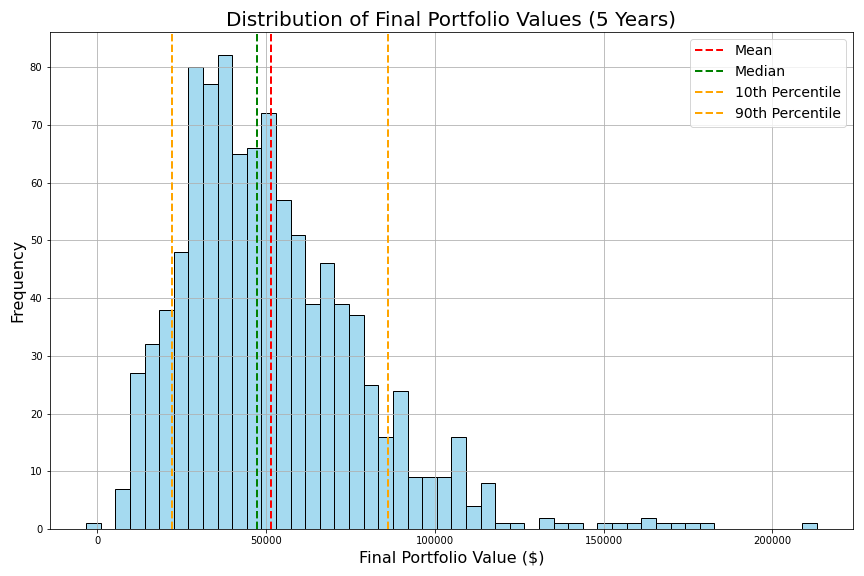
\includegraphics[width=0.8\textwidth]{../Figures/final_portfolio_values_distribution_5_years.png}
    \caption{Distribution of Final Portfolio Values (5 Years)}
    \label{fig:final_portfolio_values_5y}
    \subcaption{The histogram displays the distribution of final portfolio values after a 5-year investment horizon. Vertical lines indicate the mean, median, 10th percentile, and 90th percentile values.}
\end{figure}
\FloatBarrier

\begin{figure}[!htbp]
    \centering
    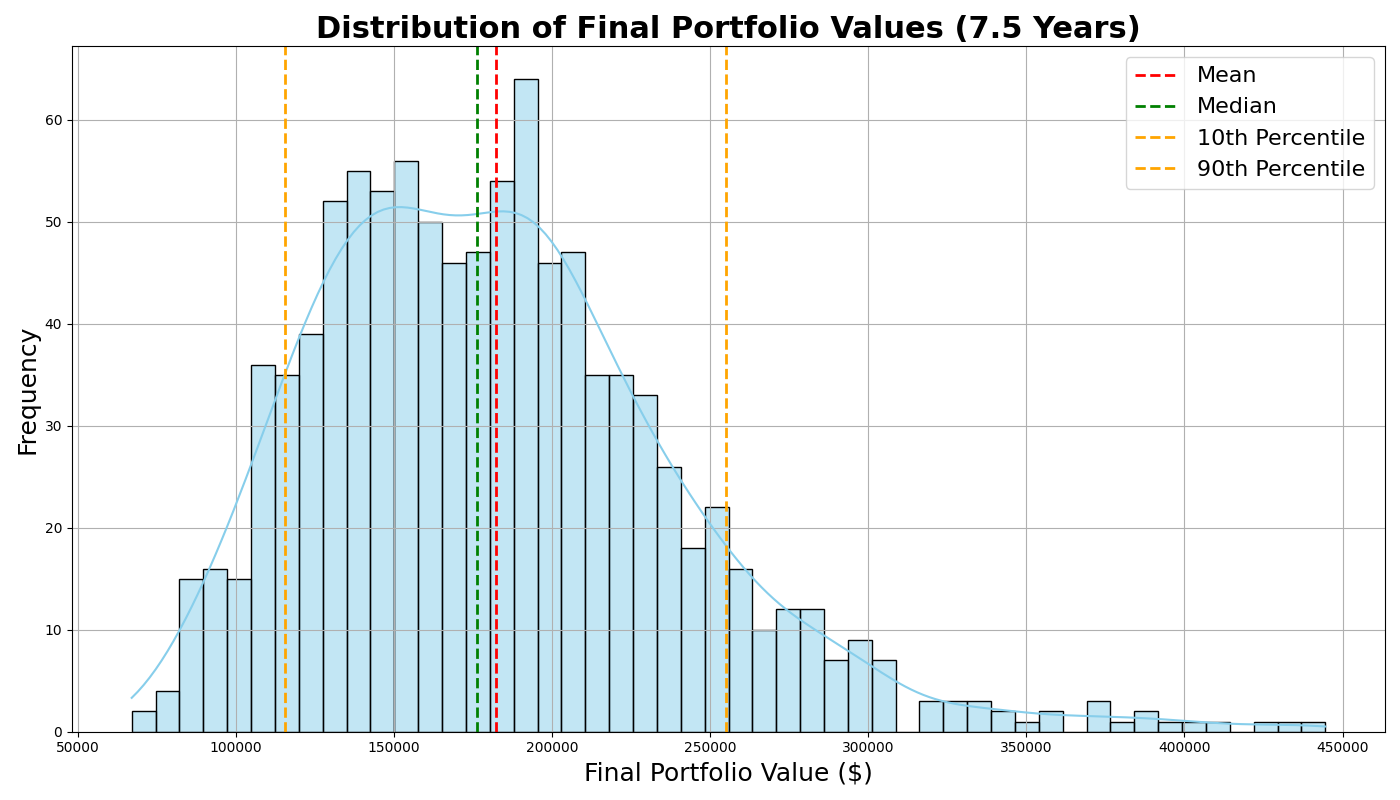
\includegraphics[width=0.8\textwidth]{../Figures/final_portfolio_values_distribution_7_5_years.png}
    \caption{Distribution of Final Portfolio Values (7.5 Years)}
    \label{fig:final_portfolio_values_7_5y}
\end{figure}
\FloatBarrier

\begin{figure}[!htbp]
    \centering
    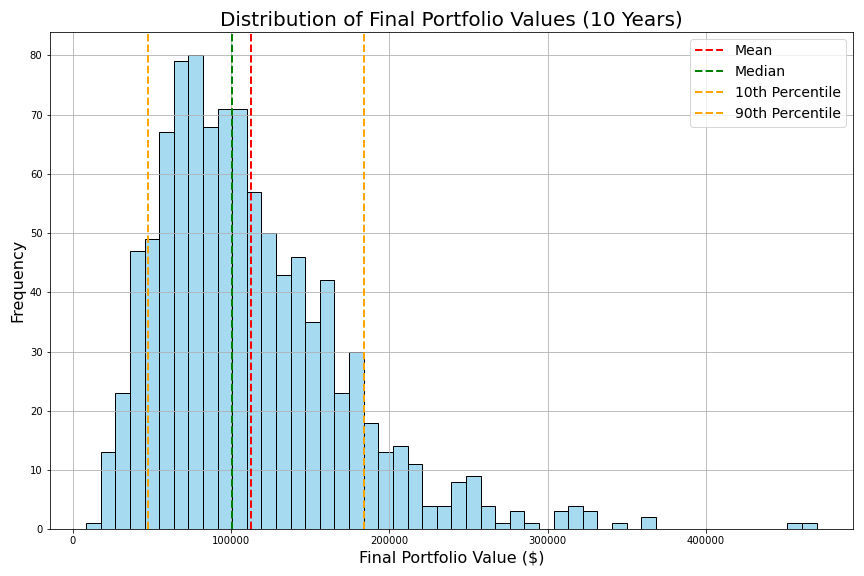
\includegraphics[width=0.7\textwidth]{../Figures/final_portfolio_values_distribution_10_years.png}
    \caption{Distribution of Final Portfolio Values (10 Years)}
    \label{fig:final_portfolio_values_10y}
\end{figure}
\FloatBarrier

\subsection{Monte Carlo Forecast Summary}

\begin{table}[h!]
\centering
\scriptsize
\begin{tabular}{lccccccc}
\hline
Statistic & \begin{tabular}[c]{@{}c@{}}Mean Final \\ Portfolio Value (\$)\end{tabular} & \begin{tabular}[c]{@{}c@{}}Median Final \\ Portfolio Value (\$)\end{tabular} & \begin{tabular}[c]{@{}c@{}}10th Percentile Final \\ Portfolio Value (\$)\end{tabular} & \begin{tabular}[c]{@{}c@{}}90th Percentile Final \\ Portfolio Value (\$)\end{tabular} & \begin{tabular}[c]{@{}c@{}}Total Percentage \\ Yield (\%)\end{tabular} & \begin{tabular}[c]{@{}c@{}}Annual Percentage \\ Yield (\%)\end{tabular} \\
\hline
10-Year Horizon & 283094.44 & 265864.65 & 171232.59 & 420935.51 & 2730.94 & 39.70 \\
7.5-Year Horizon & 180745.35 & 173433.88 & 116972.91 & 256760.32 & 1707.45 & 47.10 \\
5-Year Horizon & 101559.42 & 98327.18 & 67062.20 & 139233.79 & 915.59 & 58.98 \\
\hline
\end{tabular}
\caption{Summary statistics of final portfolio values across different investment horizons (5, 7.5, and 10 years). The table includes mean, median, 10th percentile, and 90th percentile final portfolio values, as well as the total and annual percentage yields for each investment horizon.}
\label{table:summary_statistics}
\end{table}
\FloatBarrier

\section{Results Summary}

The analysis of optimal investment strategies for first-time homebuyers provides several key insights. Stocks consistently outperform ETFs and mutual funds, underscoring their long-term growth potential. This is confirmed by the exploratory data analysis. In the 5-year horizon, top assets include airlines like AAL, DAL, and ALK, indicating strong short-term growth potential. The 7.5-year horizon features a diverse mix of technology, finance, and industrial sectors. In contrast, the 10-year horizon is dominated by financial and industrial stocks such as Fidelity Blue Chip Growth Fund, Kimberly-Clark, and NextEra Energy, showcasing significant long-term growth potential.

Optimal portfolio allocation using Modern Portfolio Theory (MPT) mirrors these trends. The 5-year portfolio balances stocks and mutual funds, favoring T. Rowe Price Health Sciences Fund and Sempra Energy. The 7.5-year portfolio is mainly composed of ETFs containing NASDAQ-100 and healthcare securities, along with key stocks such as Altria. For the 10-year horizon, the portfolio is primarily stocks, with significant holdings in Fidelity Blue Chip Growth Fund, Kimberly-Clark, and NextEra Energy, demonstrating the effectiveness of a long-term strategy.

The cumulative returns comparison indicates that the 5-year horizon portfolio achieves the highest returns, significantly outperforming the S\&P 500. The 10-year horizon, while still achieving substantial gains, comes in second place, demonstrating the benefits of long-term investment. The 7.5-year horizon, although yielding considerable returns, ranks third. This highlights the remarkable performance of the 5-year portfolio, even at lower percentiles, showcasing its robustness. The mean final portfolio values further confirm these findings, with the 5-year horizon showing impressive returns, the 10-year horizon reflecting substantial growth potential, and the 7.5-year horizon indicating better performance over a medium-term horizon.

Cumulative returns over time using Monte Carlo Simulation display consistent growth. The 5-year horizon shows a clear upward trend, while the 7.5-year and 10-year horizons demonstrate sustained growth resilient to market fluctuations. The summary statistics showcase the robustness and effectiveness of the optimization strategy across different market conditions and investment periods, underscoring the importance of diverse asset allocation, sectoral diversity, and the benefits of long-term investment for achieving substantial returns.


\newpage
